\newpage
\subsection{Triển khai và kết quả}

Giao diện \textit{hệ thống quản lý} được xây dựng với thư viện \href{https://reactjs.org}{\textit{React}} (được phát triển bởi đội ngũ \textit{Facebook} với sự đóng góp của cộng đồng) sử dụng ngôn ngữ lập trình \href{https://www.typescriptlang.org/}{\textit{TypeScript}}. Đồng thời, người dùng cần đồng ý kết nối ví mã hoá \textit{MetaMask} với hệ thống để sử dụng các tính năng tương tác với hợp đồng thông minh. Phía máy chủ, \href{https://nodejs.org}{\textit{Node.js}} được lựa chọn, ta sử dụng \href{https://expressjs.com/}{\textit{Express}} để tạo các \textit{API}\footnote{Application Programming Interface}. Thông tin cần thiết được lấy từ cơ sở dữ liệu, và việc trao đổi giữa máy chủ và giao diện được thực hiện qua kết nối \textit{HTTP} và \textit{Web Socket}, các cập nhật từ một người sẽ được thông báo ngay lập tức tới các cá nhân khác trong cùng cơ sở cấp phát văn bằng.\\

\textit{Hệ thống tra cứu} sử dụng cấu trúc \textit{trang tĩnh}\footnote{Static web}, triển khai trên \textit{GitHub Pages} với mã nguồn công khai, cung cấp cho người dùng một công cụ tra cứu thông tin văn bằng nhanh chóng, đáng tin cậy. Các doanh nghiệp có thể lấy danh sách \textit{địa chỉ ví} của các cơ sở giáo dục tại trang thông tin (website) của cơ sở giáo dục đó, hoặc lấy từ một cơ quan có độ tin cậy lớn (như \textit{Bộ Giáo dục và Đào tạo} chẳng hạn). Thông tin số hiệu văn bằng sẽ được ứng viên cung cấp.\\

Dưới đây là một số hình ảnh khi người dùng trải nghiệm hệ thống, và em xin lưu ý \textit{đây chưa phải là hình ảnh của hệ thống hoàn thiện}.\\

\begin{figure}[!ht]
    \centering
    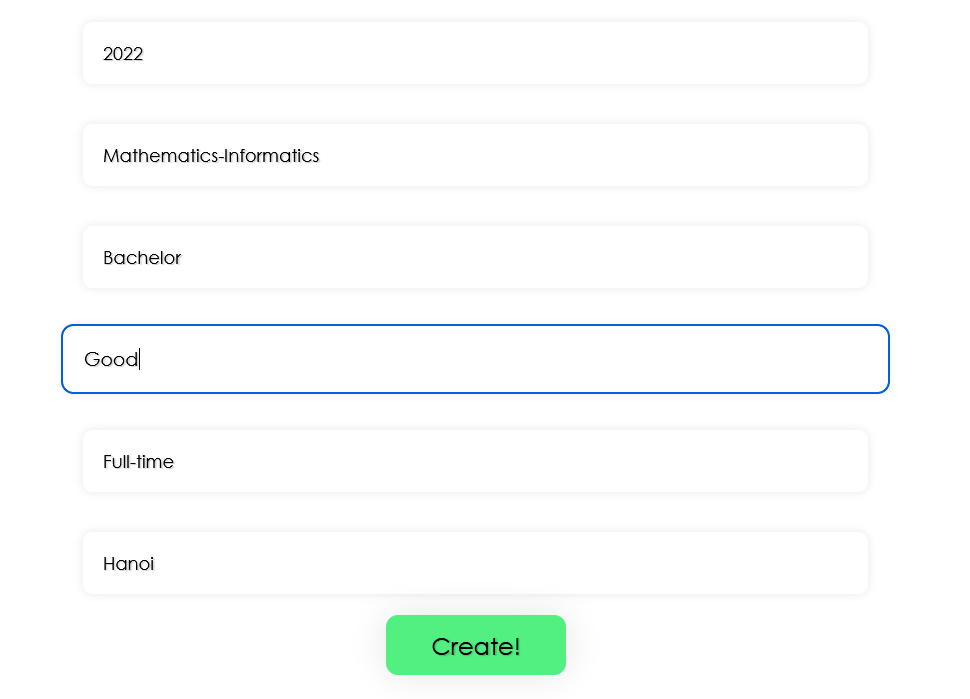
\includegraphics[width=300px]{images/app-create-cert.png}
    \caption{Một phần giao diện thêm văn bằng}
\end{figure}

\begin{figure}[!ht]
    \centering
    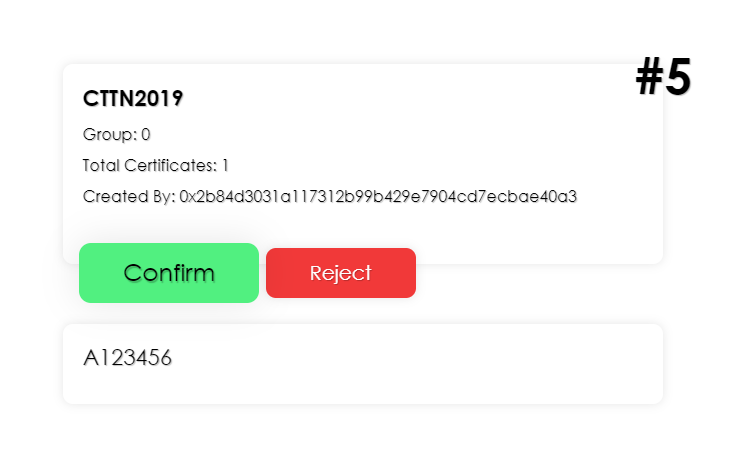
\includegraphics[width=300px]{images/app-confirm-cert.png}
    \caption{Một phần giao diện biểu quyết thêm văn bằng}
\end{figure}

\begin{figure}[!ht]
    \centering
    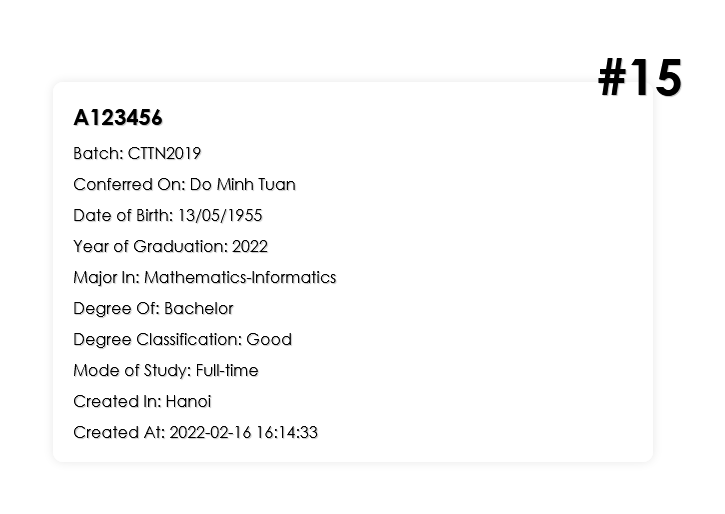
\includegraphics[width=300px]{images/app-cert-info.png}
    \caption{Một phần giao diện thông tin văn bằng đã được thêm}
\end{figure}

\begin{figure}[!ht]
    \centering
    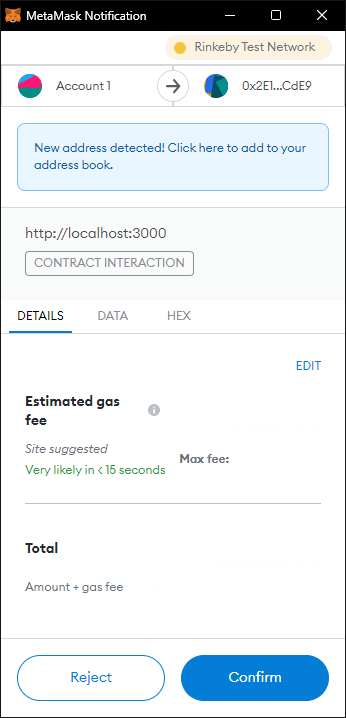
\includegraphics[width=200px]{images/metamask-confirm-cert.png}
    \caption{Giao diện MetaMask tương tác với hợp đồng thông minh}
\end{figure}

\begin{figure}[!ht]
    \centering
    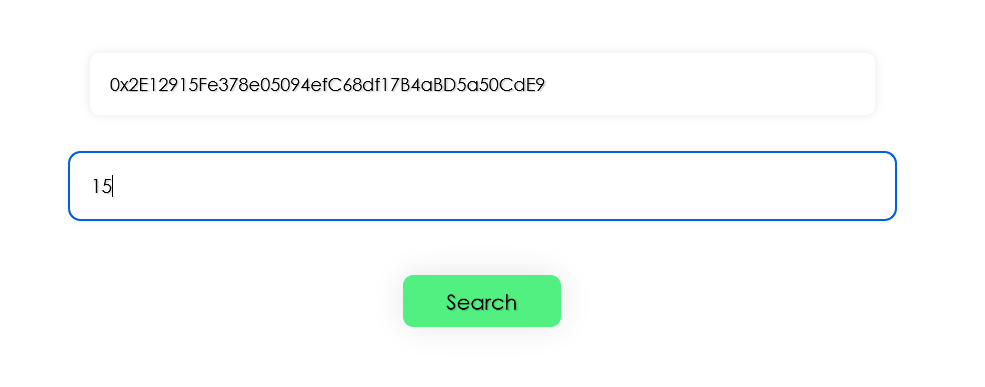
\includegraphics[width=300px]{images/app-look-up-cert.png}
    \caption{Một phần giao diện tra cứu văn bằng}
\end{figure}

\begin{figure}[!ht]
    \centering
    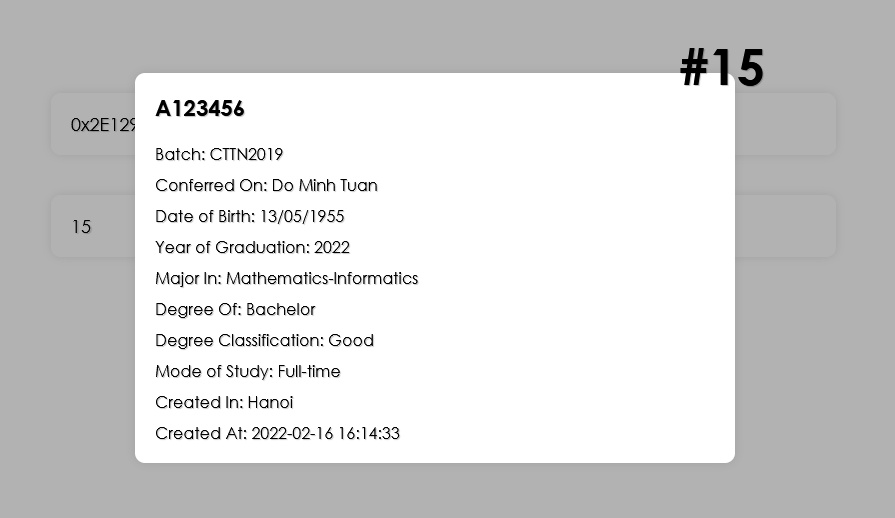
\includegraphics[width=300px]{images/app-look-up-cert-found.png}
    \caption{Một phần giao diện thông tin văn bằng khi tra cứu}
\end{figure}